\documentclass[english,a4paper]{report}
%\usepackage[margin=2cm]{geometry}
\usepackage[T1]{fontenc}
\usepackage[latin9]{inputenc}
\usepackage{graphicx}
\usepackage{babel}
\usepackage{listings}
\usepackage{verbatimbox}
\usepackage{apacite}
\usepackage{subcaption}
\usepackage{url}
\usepackage{bytefield}
\usepackage{color}
\usepackage{enumitem}
\usepackage{tikz}
\usepackage[toc,page]{appendix}
\usepackage{forest}
\usepackage{titling}
\usepackage{amsmath}
\usepackage{pgfplots}
\usepackage[affil-it]{authblk}

% reset counter per chapter
\usepackage{chngcntr}
\counterwithin{figure}{chapter}

\renewcommand{\lstlistingname}{Listing}
\usepackage{courier}
% make lstlisting use monospace fonts
\lstset{basicstyle=\footnotesize\ttfamily,breaklines=true}
\lstset{framextopmargin=50pt}

\pretitle{%
  \begin{center}
  \LARGE
  \rule[0.5ex]{1\columnwidth}{2pt}
   
\includegraphics[scale=0.5]{nmmu.jpg}
   \rule[0.5ex]{1\columnwidth}{2pt}
}
\posttitle{

\end{center}
}


\begin{document}

\title{A JIT-Less Type-Mapped Dynamic-ISA Virtual Machine for
  Many-Instance Applications}

\author{ Douglas Bentley \and Supervisor: Kevin Naude }

\maketitle

\begin{center}
Submitted in partial fulfilment of the degree Baccalaureus Scientiae
(Honores) in Computer Science at the Nelson Mandela Metropolitan
University
\end{center}

\newpage{}

\chapter*{Acknowledgements}

\newpage{}

\chapter*{Abstract}

\newpage{}

\chapter*{Declaration of Own Work}

\newpage{}

\listoffigures
\newpage{}

\chapter*{List of Tables}

\newpage{}

\tableofcontents
\newpage{}

\chapter{Introduction}

In the last 20 years, software applications programming has seen a
shift away from compiled languages, that run natively on hardware,
towards interpreted languages that require the use of another program,
called an interpreter, to execute them. This has several
advantages. One is portability. If you have an interpreter that runs
on different hardware and operating systems you can run your
interpreted programs in these different environments with no change to
your code. Another advantage is that memory can be managed. This helps
prevent bugs and security issues and takes the burden of managing
memory off the programmer. The disadvantage of interpreted languages
is that they must necessarily be slower than equivalent native
code. For systems programming and big-budget video games, natively
compiled languages are preferred as the performance hit is considered
to be too great but for general applications programming interpreted
languages are preferred. For business systems this usually means Java
and C\# and for web development this means JavaScript and PHP.

Given the popularity of these languages, research into interpretershatter
performance is important.

\section{Dynamically Typed Languages}
Dynamically typed languages are the foundation on which the modern
website is built. Currently there are two major web-development
languages: JavaScript and PHP. All major browsers have JavaScript
engines (virtual machines) which can interpret and execute JavaScript
code. Developers use JavaScript to create interactive websites. PHP on
the other hand is the most commonly used language for server-side
scripting. This is what allows web pages to have dynamic
content. Pages can be generated as needed and personalised for each
user using PHP. Several other dynamically typed languages are commonly
used for server-side scripting. These include Ruby (Ruby on Rails),
Python (Django) and JavaScript (Node.js).

Dynamically typed languages also play the role of ``glue'' languages
that stick together different software components. A prime example is
the Lua programming language which is used for video game
scripting. In this instance the video game's engine is written in C++
for better performance but the logic of the game is a Lua script that
runs on the Lua virtual machine. Since Lua is a higher-level language
it can be used to more easily and succinctly express the less
performance-critical elements of the game. Another example is the Bash
command language which acts as ``glue'' for the GNU core utilities
which are written in C. Each program in the coreutils performs a
simple operation but these can easily be composed using a Bash script
or command to create complex behaviour. Dynamic languages are ideal
for tasks like this because they have simple, terse syntax and
powerful abstractions.

\section{Interpreting Dynamically Typed Languages}
Dynamically typed languages are commonly paired with an
interpreter. That is, these languages are not compiled to machine code
that can be run on some architecture. Instead, it is the job of a
seperate program to determine the meaning of the program and perform
the instructions on actual hardware. There are three main approaches
to interpreting dynamically typed languages:

\subsection{Line by Line}
In line by line interpretation the program is parsed one line at a
time. Each line is executed before moving on to the next line in the
program. This is ideal for command-line interface operating systems
where the primary mode of interaction is entering single-line
commands. Some examples of langauges with this type of interpreter
are: Bash, CMD.EXE, Python and Ruby.

\subsection{Abstract Syntax Tree}
Abstract syntax tree or AST interpreters parse the entire program and
build an abstract syntax tree that represents the structure of the
program. This tree can then be traversed in the correct order to
execute the program. The abstract syntax tree has a node for each
construct in the abstract syntax of the programming
language. Arithmetic operations are nodes for example where each
branch off them is an expression or constant.

Figure~\ref{fig:ast} shows an abstract syntax tree for an if
statement. The if statement has three branches: one for the condition,
one for the set of statements to perform if the condition is true and
another for the set of statements to perform if the condition is
false. By traversing to the first branch of the ``if'' node and then
to the second or third given the condition, the value of the variable
``max'' can be calculated. An entire program can be parsed into an AST
and interpreted in this fashion.


\begin{figure}
  \begin{subfigure}{.5\textwidth}
    \begin{lstlisting}
      if (x > y)
          max = x;
      else
          max = y;
    \end{lstlisting}
    \caption{If statement code}
  \end{subfigure}
  \begin{subfigure}{.5\textwidth}
    \centering

    \begin{forest}
      for tree={ draw, s sep=6mm } [if [> [x][y]] [{=} [max] [x]]
      [{=}[max] [y]]]
    \end{forest}

    \caption{Tree parsed from code}
  \end{subfigure}
  \caption{Abstract Syntax Tree \protect\cite{ast}}
  \label{fig:ast}
\end{figure}


\subsection{Bytecode}
Bytecode interpreters interpret a pre-compiled bytecode that is much
like the machine code executed by the CPU. An additional tool called a
compiler is needed to generate the bytecode from the program's text.

\begin{figure}
  \centering
  
  \caption{Bytecode}
  \label{fig:byte}
\end{figure}

This can be stored compactly and executed by decoding the opcode and
performing the instruction associated with it. This approach is found
in the statically typed languages Java and C\# but dynamically typed
languages like Lua share the same approach. Bytecode interpreters are
also called virtual machines because of they perform the same tasks as
a real CPU: fetching, decoding and executing instructions (citation
needed?).

The Lua bytecode (as of Lua 5.0) is made up of 32-bit unsiged integers
\cite{RobertoIerusalimschy}. Figure~\ref{fig:luabyte} shows the
different ways the bits of the instructions in the bytecode are
used. Bits 0 through 5 are always used to store the opcode. Bits 6
through 13 are always used to store the first argument. After that
there are three options for how the rest of the instruction word is
used.

\begin{figure}
  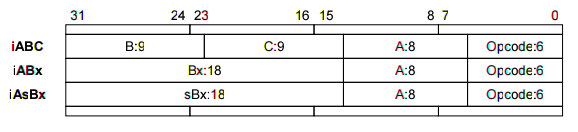
\includegraphics[width=\linewidth]{luabytecode.png}
  \caption{Lua VM bytecode layouts
    \protect\cite{RobertoIerusalimschy}}
  \label{fig:luabyte}
\end{figure}

\section{Organisation of a Virtual Machine} 
A Virtual Machine executes a binary file that is a list of
instructions in the bytecode format for that Virtual Machine. So for
Lua these instructions would be 32-bit integers in one of the formats
seen in Figure~\ref{fig:luabyte}. The binary file may also contain
data for known constant values in the program.

\subsection{Instruction Pointer}
When executing bytecode, the virtual machine needs some way to know
what instruction is currently being executed. This is slightly more
complex than just keeping track of how far into the program the VM has
read as the program may have ``control flow'' instructions. These
instructions allow the virtual machine to jump between different
points in the program. This is how loops and conditional execution are
implemented.

The instruction pointer (or IP) is used for this purpose. Its only
purpose is to point to the current instruction.

\subsection{Instruction Set}
Each VM has a set of subroutines called the instruction set. Each
subroutine performs a specific function necessary for the execution of
a program. A VM usually has instructions for performing arithmetic
operations (\verb|add|, \verb|divide|, \verb|subtract| ...), bit
manipulation operations (\verb|xor|, \verb|and|, \verb|or| ...),
control flow operations (\verb|jump|, \verb|jumpif0|, ...) and for
storing and accessing values (\verb|load|, \verb|store|, ...). The
design of a VM instruction set, much like that of a CPU, is a creative
process. The particular set of instructions a virtual machine has is
the decision of the designer and choosing which instructions to
include and omit has trade-offs that need to be considered.

\subsection{Dispatch Mechanism} 
At the core of the virtual machine is its dispatch mechanism. The VM
reads the instruction that the instruction pointer points to and then
must determine what subroutine needs to be called to execute the
instruction. Selecting and moving execution to this subroutine is
called ``dispatch''. How to implement this dispatch mechanism is a
complex topic that will be discussed in more depth in chapter 3. The
dispatch mechanism also influences how the opcodes in the instruction
word are seperated from the operand.

\section{Problem Description}
Modern process virtual machines make use of JIT compilers. Both JVM
and .Net make use of a JIT compiler \cite{MSDN,Oracle}. 

For applications that run many concurrent instances, like a web server
which starts up a new process for every client, a virtual
machine that makes use of a JIT compiler defeats the benefits of
read-only memory sharing. This is because jitted code is created at 
runtime and thus is saved in the process's private memory. So jitted 
code is not shared between instances of the VM running the same 
code. 

Bytecode that has not been jitted can be shared between applications,
however. If we wish to take advantage of read-only memory sharing a
JIT-less virtual machine is needed. As was covered in chapter 2, JIT
compilation can greatly reduce the time taken to execute
programs. Thus alternative ways to increase the performance of
programs executed on the VM need to be found to counter the
performance loss of losing the JIT compiler.

\section{Project Objectives}
The objective of this project is to implement and benchmark an
experimental JIT-less virtual machine design for a dynamically typed
language. In order to benchmark the performance of the virtual machine
an additional two virtual machines must be developed. One of these is
a conventionally implemented virtual machine. The other is an
additional experimental VM needed to test the effectiveness of a
particular element of the proposed solution. This will be discussed
further in chapter XXX.

A set of benchmarks must be hand-written to run on the new virtual
machines. The running times of the benchmarks on each of the three
virtual machines must be compared and analysed. The project aims to
determine what kind of performance benefits (if any) can be attained
by the two experimental implementations over the conventionally
designed virtual machine.

\section{Project Scope}

The VMs are experimental prototypes, hence several tools and features
conventionally paired with a VM are considered out of scope for this
project. There will be no \textbf{compiler} or \textbf{assembler}
implementation required and the VM will not be required to perform
\textbf{garbage collection}.

\begin{itemize}
\item A compiler implementation is unnecessary as the VM designs are
  experimental prototyped and are not meant for further use, thus
  benchmarks can be hand-written as they are the only programs needed
  to run on the virtual machine. Similarly, robust error handling and
  debugging tools are considered out of scope.
	
\item An assembler will be used to make writing benchmarks more
  bearable but is not considered in scope as it is simply a tool used
  to facilitate easier writing of benchmarks and not an important part
  of the implementation of the virtual machine.
	
\item Garbage collection is considered out of scope because the
  implementation of a garbage collector adds to the complexity of the
  project and may influence the results of running the benchmarks. A
  GC is also unnecessary to run the benchmarks.
\end{itemize}


%floating point and advanced threading techniques

\section{Risks}
The risks of the project are mainly about its structure and how it can
be criticised. The VM will be running predefined benchmarks. If it
performs those well at the expense of its general usefulness the
project can be criticised. All of these sorts of criticisms can be
mitigated so long as the goal of the project is kept in mind at all
times. Learning as much as possible about how well the idea works
should always take precedence over trying to make results look
good. Whether the VM performs better or not is important knowledge and
being as careful as possible about discovering that accurately is
extremely important.

A risk mitigated by the design of the study is that the hand-written
benchmarks may not be optimised as well as those produced by a
compiler. Since all three VMs will run identical benchmarks this risk
is mitigated because any lack of optimisation in a benchmark
experienced by one VM will be experienced by all other VMs. Comparing
the experimental VMs with an existing conventional VM design would be
ineffectual as it may perform better purely because the code produced
by the compiler is better optimised.

\section{Overview of Treatise}
In chapter 2, the virtual machine as a concept will be introduced and
the different types of virtual machines will be covered. Existing
solutions to the problem of a VM for dynamically typed language will
be examined and some theory about modern processors will be
covered. This theory informs some of the design decisions of the
virtual machine.

In chapter 3, the design of the VM will be covered. This chapter will
cover how the VM works, what instructions it supports and discusses
why certain design decisions were made given the information in
chapter 2.

In chapter 4, the implementation details of the VM are covered, with
code samples provided as examples for various important elements of
the VM's design like dispatch, function calls and how instructions are
implemented.

In chapter 5, the experimental design and benchmarks will be
discussed. Which benchmarks were chosen and what they can tell us
about the virtual machine will be discussed in this chapter. It will
also detail the exact details of how the experiment was conducted so
that it may be repeatable with similar hardware.

In chapter 6, the results of the experiment will be discussed and
analysed and the performance benefits of the virtual machine will be
examined.

Lastly in chapter 7, conclusions will be drawn about in what instances
the implementation for the virtual machine is useful and what its
strengths and weaknesses are.
\newpage{}

\chapter{Background and Literature Review}
This novel virtual machine is called the \textbf{Operand-Type Dispatch
  VM} or just the \textbf{Operand-Type VM}. Its placement in the
heirarchy of virtual machines is examined in this section.

A review of existing systems, modern processor architectures and
current literature on virtual machine design is necessary as these
elements inform the design decisions made for the \textbf{Operand-Type
  Dispatch VM}.

\section{Virtual Machines}
A \textbf{virtual machine} or \textbf{VM} is a computer program that
``executes software in the same manner as the machine for which the
software was developed'' \cite[pg9]{JamesE.Smith2005}. This program is
designed to run on some real machine. We call the real machine that a
virtual machine is running on the \textbf{host} and the virtual
machine the \textbf{guest}. The guest machine provides an execution
environment for software that is designed to run either on the guest
itself or on an actual machine that the virtual machine is
emulating. This means that we can use a virtual machine to run
programs that are incompatable with the host. The virtual machine
allows this by providing a mapping of its state to the state of the
host machine on which it is running \cite[pg4]{JamesE.Smith2005}.

\section{The Types of Virtual Machines}
Virtual machines come in two varieties: \textbf{process} virtual
machines and \textbf{system} virtual machines.

A process virtual machine is ``capable of supporting an individual
process''\cite[pg9]{JamesE.Smith2005}. This means that the host runs
the guest for as long as a single process on the guest machine needs
it. Once the process has completed its execution the guest machine
terminates\cite[pg9]{JamesE.Smith2005}. An example of a process
virtual machine is the Java Virtual Machine or JVM. All java programs
run on the JVM. An instance of the JVM is started when you execute a
java program and killed when its execution is complete.

A system virtual machine ``provides a complete system environment''
''\cite[pg9]{JamesE.Smith2005}. This means that it can support an
entire operating system on the guest machine and the many processes
that the guest operating system executes. A system virtual machine
will terminate when the guest system is shut down.

\section{The Types of Process Virtual Machines}

Process virtual machines can be divided into two categories:
\textbf{multiprogrammed systems} and \textbf{dynamic}
\textbf{translators}. The difference between these is whether or not the
guest machine uses the same instruction set architecture as the host
machine.

With multiprogramming the guest and host use the same instruction
set. Multiprogramming is supported by most operating systems and
allows a user to run many processes at once by ``making each process
think it has access to an entire machine instead of only part of a
machine''\cite[pg13]{JamesE.Smith2005}. The OS creates an environment
per process that it terminates when that process ends execution.

With dynamic translators the instruction set of the host and guest
generally do not match. The virtual machine translates blocks of
instructions meant for the machine it is emulating and translates them
into instructions to be run on the host. Not all code is translated in
a dynamic translater. Only code that is used often enough will be
translated as there is an overhead involved with translating code. The
code that is not translated is interpreted. Interpreted instructions
are read, their meaning interpreted and then executed. This
interpretation step must happen each time a piece of code is executed
so code that is executed enough times will be dynamically translated
and cached so later execution is faster. Dynamically translating in
this manner is known as \textbf{just-in-time compilation} (JIT
compilation).

\section{Where the Operand-Type Dispatch VM is Situated}
The Operand-Type VM is a process virtual machine. It has a new
instruction set architecture and hence is different from any host
machine's ISA. The Operand-Type VM is exclusively an interpreter and
does not make use of a JIT compiler. It is designed to run processes
written in a dynamically typed languages. For these reasons it is a
``JIT-less'', ``Dynamic-ISA'' virtual machine. 

\section{Dynamic vs Statically Typed Programming Languages}
A dynamically typed language is one in which the type information is
associated with values \cite[pg4]{RobertoIerusalimschy}. An example of
a dynamically typed language is JavaScript. In JavaScript the var
keyword is used for variables. This is because the type is associated
with the value stored in the variable so variables themselves need not
be told which type is associated with them. Any variable can hold a
value of any type. A statically typed language is one in which the
type information is associated with the variable. An example of this
is Java. In Java variables are declared using keywords that define
their type (\textbf{int}, \textbf{String} etc). Each variable can only
hold a value of that type. Each approach has its strengths and
weaknesses.

\subsection{Type Safety }
With static typing a program's type correctness can be checked at
compile time. Because the types of all variables are known when the
code is written, operations on those variables can be declared valid
or invalid when code is compiled. If an operation that acts on one
type of variable is given another the program will not compile. This
knowledge is advantageous for the programmer and for the machine (or
VM as the case may be).

The programmer benefits from knowing whether or not his program is
correct at compile time. The implications of this are larger than just
being able to find errors while compiling some piece of code instead
of while running it. A type error in a dynamically typed language has
to actually be executed before it can be detected. If a type error
occurs in a rarely taken path of execution in a dynamically typed
program, it may not be detected at all. This means that a programmer
writing in a dynamically typed language must ensure that the values in
the variables they use are of types that make sense for the operations
they wish to perform. A programmer writing in a statically typed
language will have their types checked for them.

Figure \pageref{fig:dvs} shows how Java, a statically typed language
and Lua, a dynamically typed language, handle code which tries to
perform addition of two types that cannot be added in either
language. The Lua code compiles but encounters an error at
runtime. The Java code does not compile.

The machine or VM benefits from not having to check the types of
instruction arguments. This is a major overhead in dynamically typed
languages. In a dynamically typed language, the types of the arguments
must be checked for each instruction the VM or machine must perform as
all arguments are values. This means that an addition instruction that
works on integers, for instance, must check that the values it is
trying to add are in fact integers before it can add them.

\begin{figure}
  \begin{subfigure}{.48\textwidth}
    \begin{lstlisting}
      class main {
        public static void main(String[] args) {
          int foo = 12;
          String bar = ``bar'';
          int foobar = foo + bar;
        }
      }
    \end{lstlisting}
    \caption{Java: does not compile}
  \end{subfigure}
  \begin{subfigure}{.48\textwidth}
    \begin{lstlisting}
      foo = 12
      bar = ``bar''
      foobar = foo + bar
    \end{lstlisting}
    \caption{Lua: compiles but encounters error}
  \end{subfigure}
  \caption{Dynamically vs Statically Typed Languages}
  \label{fig:dvs}
\end{figure}

\section{Advantages of Dynamically Typed Languages} 
Dynamically typed languages have their own advantages. Programs
written in dynamically typed languages tend to be shorter than
equivalent programs written in statically typed languages and
dynamically typed languages are considered to be easier to prototype
ideas in. Also, a subset of logically correct programs will not be
accepted by a statically typed language's type checker. Dynamic typed
languages allow the freedom to write these kinds of programs.

Dynamically typed languages are also powerful for handling arbitrary
data. This is exemplified by the JSON format, based on JavaScript. An
arbitrary database query for an application in a statically typed
language often has to be mapped to an object for some static class and
the types of the values placed into that object have to be checked
anyway. for these types of problems a dynamically typed language can
build arbitrary objects on the fly.

Of course statically and dynamically typed languages can be realised
in many different ways. Both dynamic and statically typed languages
are widely used and so VM research for both statically and dynamically
typed languages is important.

\section{Modern Processor Architecture}

In order to create an efficient VM, we need first understand how
modern processors work and what some of the bottlenecks for our VM's
execution might be. For example, \textbf{threading techniques} (not to
be confused with threads in application programming) are commonly used
in VM design. These take advantage of a feature of modern processors
called the \textbf{Branch Target Buffer} or BTB. The BTB exists to aid a
process called \textbf{branch prediction}. Branch prediction itself can
only be explained once we know about how modern processors make use of
\textbf{pipelining} to increase their throughput. As you can see, an
understanding of modern computer architectures is needed before we can
begin a discussion of VM design.

\subsection{Pipelining}

Pipelining is a process in which a processor's instruction processing
cycle is shared by many consecutive instructions at once. The
instruction processing procedure is split up into smaller stages that
can execute simultaneously. An example of this is the classic RISC
pipeline which divides instruction processing into the following
steps: Instruction Fetch (IF), Decode (ID), Execute(EX), Memory Access
(MEM) and Writeback (WB). Each instruction passes a stage and leaves
that part of the processor free to perform that stage on the next
instruction. Thus many instructions (as many as there are stages) can
be processed at once, instead of each instruction having to be
completely processed before the processor is free to move onto the
next instruction. The process is analogous to an asssembly line, where
many cars can be assembled at the same time, each in a different stage
of assembly.

\begin{figure}[tph]
  \centering
  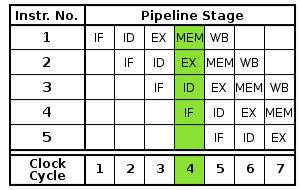
\includegraphics[scale=0.5]{pipeline}
  \caption{Simplified CPU pipeline}
  \label{fig:pipeline}
\end{figure}

In figure~\ref{fig:pipeline} we see that the first instruction as
currently performing memory access while the second EXecutes and the
third is being Decoded. Up to 5 instructions can be processed
simultaneously.

When pipelining an interesting situation occurs in the case of some
control flow instructions. Control flow instructions are those that
cause execution to move to some other point in the program. For
control flow instructions where the jump is conditional (based on some
criteria being true) the point at which we know which instruction
comes next (called \textbf{branch resolution}) is usually later in the
pipeline. Thus the processor cannot queue up the next instruction as
it does not know which instruction will execute next. Branch
prediction is used in modern processors to try to keep the pipeline as
full as possible and not waste time waiting for this information to be
known.

\subsection{Branch Prediction}

Instead of filling up the pipeline with no operation instructions
until we know where to branch, with branch prediction we guess which
branch will be taken and place the instructions from the predicted
branch into the pipeline. When we know where the branch operation
should have taken execution we either throw out our newly pipelined
instructions (this is called \textbf{pipeline flushing}) if the
prediction was incorrect or continue execution if it was correct.

The more stages the pipeline has before branch resolution, the more of
a performance benefit correct predictions become for programs with
many conditional control flow instructions. A Virtual Machine is such
a program. This is because a VM must branch to the correct code for
each instruction it executes. Writing code that allows for increased
branch prediction accuracy is thus important for VM efficiency.

Predicting a branch means we must predict if that branch is taken or
not and what the target of that branch is if it is taken. Modern
processors have a Branch Target Buffer where the target adresses of
previously taken branches are cached. So upon arrival at a branch that
has been previously taken, we guess if it will be taken and begin
speculatively executing from the address stored in the BTB.

\subsection{Cache}

Modern processors make use of different levels of cache to allow for
faster memory access. Ideally we would like to have an infinite amount
of memory with no time cost for accessing it. The reality is that the
larger memory is, the slower it becomes to access it. In order to get
closer to the ideal modern processors make use of cache. It takes
around 100 cycles for Intel's i7-4720HQ (Haswell) architecture to
access memory. Cache allows us get get closer to the ideal case by
keeping commonly accessed memory closer to the CPU in levels of
increasingly smaller, faster and more expensive (to manufacture)
memory. 

The Haswell architecture has 32KB of L1 data cache and 32KB of L1
instruction cache. These are located on the CPU itself. L1 data cache
can be accessed in around 4 cycles \cite{7-cpu}. It also has 256KB of
L2 cache and 8 MB of L3 cache. L2 cache can be accessed in 12 cycles
and L3 in about 36 cycles \cite{7-cpu}. Caching works on the principal
of locality of reference. There are two types of locality of
reference: spacial locality and temoporal locality.

Temporal locality takes advantage of the likelihood that similar data
will be needed in the near future. If some data has been accessed
recently it is cached because it is quite likely it will be needed
again soon.

Spacial locality takes advantage of the likelihood that similar data
will be needed in the near vicinity of an accessed value. Data near an
accessed value is cached because it is likely that it will be
needed. This would be good for something like sequential array lookups
because more of the array will be cached for faster access later. 

With knowledge of how cache functions we can implement a VM that makes
effective use of the processor's cache.

\section{Conventional Implementation of High Level VMs}

Several common patterns are found in the design of Virtual
Machines. Different techniques for threading the flow of execution
through the VM have been well-examined and the trade-offs between
register and stack-based VMs have been discussed and studied.

\subsection{Dispatch and Threading}

Dispatch is the process of fetching, decoding and starting the next
instruction to be run by a virtual machine.

The simplest way to implement a virtual machine is to make use of a
switch statement in a loop. This is called switch dispatch. See
figure~\ref{fig:switch} for a C implementation.

\begin{figure}
  \begin{lstlisting}
typedef enum { add /* ... */ } Inst; 

void engine() 
{ 
    static Inst program[] = { add /* ... */ }; 
    Inst *ip = program; 
    int *sp; 

    for (;;) 
        switch (*ip++) 
        { 
        case add: 
            sp[1]=sp[0]+sp[1]; 
            sp++; 
        break; 
        /* ... */ 
    }
} 
  \end{lstlisting}
  \caption{Switch Dispatch}
  \label{fig:switch}
\end{figure}

This approach is problematic because the switch statement means that
there is only ever a single entry in the Branch Target Buffer used for
dispatch . This means that the number of mispredictions will be large
as the target of the branch will change for each new instruction we
branch to. This problem may even be magnified by the fact that this
specific VM implementation has far more instructions than usual as it
requires several specialised versions of every instruction.

\begin{comment}The name threading comes from the idea of the execution
  threading its way from one instruction to the next {[}??{]}
\end{comment}

A faster alternative to switch dispatch is direct
threading\cite{Ertl}. In direct threading the program is stored as a
list of addresses of instructions and the code for each instruction
includes a dispatch portion which jumps to the address of the next
instruction to be executed.

\begin{figure}
  \begin{lstlisting}
typedef void *Inst; 

void engine() 
{ 
    static Inst program[] = { &&add /* ... */ }; 
    Inst *ip = program; 
    int *sp; 
    goto *ip++; /* dispatch first VM inst. */ 
add: 
    sp[1]=sp[0]+sp[1]; 
    sp++; 
    goto *ip++; /* dispatch next VM inst. */ 
}
  \end{lstlisting}
  \caption{Direct Threaded Dispatch}
  \label{fig:direct}
\end{figure}

Another method is indirect threading. In indirect threading we keep a
lookup table of the addresses of code for each instruction and have
each instruction jump to the next by reading the opcode of the next
instruction from the program, looking up the address of the code for
that instruction in the table and then jumping to that instruction.

\begin{figure}
  \begin{lstlisting}
typedef void *Inst;
void engine() 
{ 
    static Inst lookup[] = { &&add, &&sub /*...*/ }
    static int program[] = { 0, /* ... */ }; 
    int *ip = program; 
    int *sp; 	
    goto *ip++; /* dispatch first VM inst. */ 
add: 
    sp[1]=sp[0]+sp[1]; 
    sp++; 
    goto lookup[*ip++]; /* dispatch next VM inst. */ 
}
  \end{lstlisting}
  \caption{Indirect Threaded Dispatch}
  \label{fig:indirect}
\end{figure}

Direct and inderect threading make much better use of the branch
target buffer. Instead of a single entry in the BTB, with direct
threading we have an entry per instruction, so instructions that
commonly follow each other have a better chance of being predicted.

All code in this section is from or adapted from \cite{Ertl}.


\subsection{Registers VS Stacks}
In a stack virtual machine, instructions act on members of the
stack. Arguments and return values for instructions are often implicit
and thus instructions can be smaller. For instance a stack
implementation of a = b + c would first push b and c onto the stack,
then call the add instruction which has no arguments. Add pops b and c
off the stack and pushes b+c back onto the stack. This value is then
popped off the stack and stored.

For a register machine, a similar piece of code would have values for
b and c in registers and an add instruction is called with a, b and c
as arguments. This instruction would compute b+c and store it in a
regsiter.

Widely used process virtual machines make use of a stack
architecture. Both the Java Virtual Machine (JVM) and Microsoft's
Common Language Runtime (CLR) make use of stack virtual machines
\cite{CLI}\cite{JVM}.

\subsection{Just in Time Compilation}

Both the Hotspot Java Virtual Machine and .Net Common Language 
Runtime make use of Just in Time compilation\cite{JJIT}. JIT 
compilation allows for code that is executed often enough to be
compiled into native machine code at runtime. This means that the 
areas of code most frequently executed in the program run much faster 
than they would otherwise and the overhead of compiling and 
optimising every single piece of code, even that which is not used 
often, is removed. Removing this overhead is important because slow 
compilation at runtime can have a visible effect for users.

\section{VM Interpreter Reseach}

\subsection{Threaded Code}

James R. Bell introduced the concept of threaded code in 1973. The
Fortran IV compiler was written to generate threaded code.\cite{Bell}
Yuhne Shi\cite{Shi2007} found that a well-implemented register VM is a
more efficient option when speed of execution is more important than
the size of the code to be executed.

Ertl and Gregg found that in their benchmarks 3.2\%\textendash 13\% of
all executed instructions were indirect branches and that switch
dispatch on an architecture with a BTB resulted in 81\%-98\% branch
prediction misses \cite{EfficientInterpreters}. They also found that
direct threading resulted in 50\%-63\% branch prediction misses.

\subsection{Abstraction Level}
\label{sec:abstraction-level}
A 2009 study\cite{Brunthaler20093} by Stefan Brunthaler classed
virtual machines as high or low abstraction level virtual machines,
where low abstraction virtual machines are ``only a thin layer above a
real machine'' and high abstraction level virtual machines where the
``operation implementation requires significantly more native
instructions than for low abstraction level''.

The study aimed to question the established thought that instruction
dispatch was the main overhead for a virtual machine. He found that
this assumption does not hold for high abstraction level VMs, but is
valid for VMs with a low abstraction level.

\subsection{Specialised Instructions}

Michael Schr{\"o}der implemented a modified version of the Lua Virtual
machine that made use of the approach of specialising instructions
based on the types of their arguments when they are first
dispatched. In order to allow this to be safe, instructions that may
change the type of the arguments for that instruction have type checks
that will despecialise the instruction if need be. This approach
achieved a 20\% speed increase on Intel machines\cite{Schroder2012}.

\section{Existing Systems}

\subsection{Lua VM}

The Lua VM is an interpreter for the dynamically typed language Lua's
bytecode. Lua is used as a scripting language in game engines
\cite{LuaUsed}. It has many implementation similarities to the VM
described in this treatise and thus is of particular interest but it
differs in its strict adherance to the ANSI C standard
\cite{RobertoIerusalimschy}. Strict adherance to the standard is
something prioritised by the Lua team for portability reasons
\cite{RobertoIerusalimschy}.
\begin{description}
\item[Dynamically typed] Lua's types are associated with its values
  and not its variables.
\item[Register-based] The Lua VM is register-based instead of the
  stack approach taken by the JVM and .NET runtime.
\item[Switch Dispatch] The Lua VM makes use of the a switch dispatch
  mechanism \cite{Lua.Source}. This is a result of its strict
  adherance to the ANSI C standard which does not allow for labels as
  values which are needed for alternative threading techniques.
\item[No JIT] The lua VM does not make use of a Just in Time compiler
  (though an independent project called luajit has provided one).
\end{description}

\subsection{HotSpot JVM and .NET runtime}
Oracle's Java Virtual Machine implementation, called HotSpot is a
high performance Virtual Machine for running java
bytecode. Microsoft's .NET runtime is a similar VM that runs the
common intermeidate language that several Microsoft-developed
languages compile to. They are implemented similarly to each other and
quite differently from the VM described in this treatise:
\begin{description}
\item[Statically Typed] Both VMs make use of static types. Types are
  associated with variables instead of values.
\item[Stack-based] Both are stack-based architectures instead of
  register-based
\item[JIT] Both VMs make use of Just in Time compilation.
\end{description}

\subsection{Dalvik VM}
The Dalvik VM executes applications written for Google's Android
operating system for phones and tablets. The common is is that JVM
bytecode is translated to Dalvik bytecode to run on the Dalvik
VM. Dalvik has been replaced by ART in Android 5.0. Unlike the JVM,
the Dalvik VM is a register machine.
\begin{description}
\item[[Statically Typed]] Dalvik VM bytecode is statically typed
\item[Register-based] The Dalvik VM makes use of a register-based
  design
\item[JIT] Dalvik VM code is jitted
\end{description}

\chapter{Solution Design}



\section{Type-Mapping and Argument Case Expansion}

A type-mapped VM is one which keeps track of the state of the types of
its registers. This is beneficial because every instruction in a
conventional VM design must first verify the types of its inputs
before it can act on them. These type checks can be eliminated with
type-mapping and instructions can be customised based on the types of
the inputs they receive. 

This is closely coupled with the idea of argument case expansion. For 
Type-Mapping to be effective the VM must dispatch on its current type 
state. This is what eliminates the type checking step. But if the VM 
does not also dispatch on the arguments for the next instruction it 
cannot know which version of the instruction is appropriate. Knowing 
which types are in which registers without knowing which registers 
are arguments for an instruction means that there is not enough 
information to specialise the instruction. With argument case 
expansion a version of each instruction for every combination of 
arguments is necessary.

\section{Proposed Solution}
The proposed solution is the Operand-Type Dispatch VM. The
Operand-Type Dispatch VM makes use of type-mapping and argument case
expansion. In order to determine the effectiveness of the solution, a
further two virtual machines are needed. A conventionally implemented
VM is needed as a control to determine the performance benefits of the
Operand-Type Dispatch VM and a further VM is needed to determine the
benefits of the type-mapping of the Operand-Type Dispatch VM over just
using argument case expansion. 

These three virtual machines lie along a scale for how specific their 
instructions are. The most specific is the Operand-Type Dispatch VM. 
The Operand Dispatch VM is less specific and the Conventional 
Dispatch VM has the least specific instructions.

The details of the designs of these three virtual machines will be 
discussed in section XXXX after design decisions common to all VMs 
have been introduced. The three virtual machines are designed to be 
as similar as possible except for the aspects that the experiment 
examines. Those elements common to all VMs shall be expanded upon 
first and those specific to each shall be examined separately. 

Any referral to the \verb|VM| or the \verb|virtual machine| used from
this point without explicitly mentioning which VM is being referred to
will apply to \emph{all} three virtual machines.

\section{Virtual Machine Design Details}

The VM is a register virtual machine. The choice of being register
based was necessary for the argument case expansion to be performed
and Yuhne Shi\cite{Shi2007} showed that register machines can give a
performance increase over equivalent stack-based VMs.

The VM has 6 general purpose registers and 3 special purpose
registers. Keeping the number of registers low is important for the
Operand-Type Dispatch and Operand Dispatch VMs. With just 6 registers,
an instruction that takes 3 arguments potentially has $6^3 = 216$
argument cases.

The VM has two primitive types: integers and pointers. Keeping the
number of types and registers low is extremely important for the
Operand-Type Dispatch VM because it affects the total number of states
the VM can take on. The Operand-Type Dispatch VM can be thought of as
creating a specialised version of the VM for every type state. With
two primitive types and 6 registers this means there are a total of
$2^6 = 64$ total states the VM can take on. Increasing the number of
primitive types by one makes that $3^6 = 729$ possible states.

The VM is for a dynamically typed language. Each register
stores 'values' and all instructions act on those values. The type of
a value is stored together with the data for that value. These are
implemented in C as tagged unions. The VM has only two types: integer
and pointer.

\section{Registers}

All virtual machines make use of 6 general purpose registers. These
registers are implemented as an array of 6 \verb|values|. These shall
be referred to as $g_0$ through $g_5$. Here `g' refers to `general
purpose'.

A further two registers are found in the VM. The instruction pointer,
which will be referred to as the \verb|IP| and the frame pointer which
will be referred to as the \verb|FP|. These are a 16-bit-integer
pointer and a value pointer respectively.

In order for 

\section{Addressing}

Instructions take operands of three types:
\begin{description}
\item[register number] These operands are numbers from 0 to 5 that
  address the six registers. For the conventional VM these are an
  explicit part of the instruction word as shown in
  Figure~\ref{fig:convinstruction}. For the other two VMs these
  operands are implicitly part of the instruction word.
\item[instruction word] This type of operand considers an instruction
  word relative to IP (usually just the next instruction word) as an
  unsigned 16-bit constant. The value of these constants will be
  referred to in the following form: $name_{16}$
\item[IP-relative addressing] This type of operand considers an
  instruction word as the \verb|IP|-relative address of a 64-bit
  unsigned integer constant. The value of the 64-bit constant will be
  referred to in the following form: $name_{64}$
\end{description}

\section{Instructions}

All virtual machines support an identical set of instructions. How
these are implemented is quite different for each VM but the
functionality of each instruction does not change between virtual
machines.

Instruction words are 16 bits long. Each instruction may have a
maximum of three register-number addressed operands. If the
instruction has multiple register-number addressed operands and a
result, the result will be stored in the register addressed by the
first operand.

In some cases, specific argument combinations for an instruction have
been removed as they produce trivial results. For instance the
subtract operation cannot be used with the same register for both
arguments. Since the result of this operation is always zero and there
already is an instruction to set a register to zero, there is no need
to include this case.

The full set of instructions may be found in appendix B.

\subsection{Arithmetic Instructions}

Arithmetic instructions provide basic arithmetic operations for
registers that contain integers. If a register that does not contain
an integer is selected, an error is signalled and the VM halts. All
arithmetic instructions increment the address of the instruction
pointer. Those that make use of a constant that is looked up in the
next instruction word increment the instruction pointer's address
again so that the \verb|IP| points to the next instruction and not the
data contained in the next word.

\begin{description}
	\item[sub] find the difference of two integer-valued registers
	
	$sub(i, j\neq i) := r _{i} \longleftarrow  r _{i} - r _{j} $ \\	
	
	\item[addc] add an integer-valued register and a 64-bit integer
	constant
	
	$addc(i, const _{64}) := r _{i} \longleftarrow  r _{i} + const 
	_{64} $ \\
\end{description}

The \verb|sub| instruction exhibits the case of a trivial instruction
call that is illegal in the bytecode. Subtracting a register's value
from itself will always produce zero. This is an unnecessary
instruction since the VM already has an instruction to place zero into
a register.

Both instructions also show off how the result of the operation is
stored in the first register-number addressed register.

\subsection{Bit Manipulation Instructions}

These instructions are for performing bitwise logical operations on
integer operands and constants. The \verb|IP| is incremented in the
same manner as for the arithmetic instructions.

\begin{description}
	\item[xor] bitwise xor two integer-valued registers
	
	$xor(i, j \neq i) := r _{i} \longleftarrow  r _{i} \textbf{ \^{} 
	} r _{j} $ \\
	
	\item[shrc] logical right shift an integer-valued register by a 
	16-bit
	integer constant
	
	$shrc(i, const _{16}) :=  r _{i} \longleftarrow  r _{i} >> const 
	_{16} $ \\	
\end{description}

Here we see another trivial case. The \verb|xor| instruction does not
allow performing bitwise xor on two numbers that are the same as this
value is always zero.

The \verb|shrc| instruction makes use of a 16-bit instruction word
after the instruction for the constant argument as a 64-bit argument
is unnecessary.

\subsection{Data Movement Instructions}
These instructions allow for values to be moved between registers.

\begin{description}
	\item[mov] move a register over another register
	
	$mov(i, j \neq i) := g_{i} \longleftarrow g_{j} $ \\
	\item[movc] move a 64-bit integer constant over a register
	
	$movc(i, const_{64}):= g_{i} \longleftarrow const_{64} $ \\
\end{description}

Note the use of the \verb|g| for the \verb|mov| and \verb|movc|
instructions. This is because moving a register over another register
is a type-independent operation.

\subsection{Memory Access}
These instructions allow for getting and setting of locals (getl,
setl), objects (geto, seto) and buffers (getb, setb).

\begin{description}
	\item[getl] get a local value indexed by a 16-bit integer 
	constant and store it in a register
	
	$getl(i, const_{16}):= g_{i} \longleftarrow mem[fp + const_{16}]$ 
	\\
	\item[seto] set a value, indexed by an integer-valued register, 
	in an
	object to that of a register
	
	$seto(i, j \neq i, k):= p_{i}[header + r_{j}*scale] 
	\longleftarrow g_{k}$ \\
	
	
\end{description}


\subsection{Control Flow Instructions}

These instructions allow for jumps in execution in the program. All
jumps are relative to the current \verb|IP| value.

\begin{description}
	\item[jmp] adds a 16-bit integer constant offset to \verb|IP|
	
	$jmp(const_{16}) := ip \longleftarrow ip + const_{16}$ \\
	\item[jmpf] adds a 64-bit integer constant offset to \verb|IP|
	
	$jmpf(const_{64}) := ip \longleftarrow ip + const_{64}$ \\	
	
	\item[jcmp] adds one of three 16-bit integer constant offsets to
	\verb|IP| depending on which case holds for two different
	integer-valued registers
	
	$jcmp(i, j\neq i,less_{16},equal_{16},greater_{16}) :=$ \\
	$ ip \longleftarrow  \\
	case :r_{i} < r_{j}: ip + less_{16}   \\
	case :r_{i} = r_{j}: ip + equal_{16} \\
	case :r_{i} > r_{j}: ip + greater_{16}$ \\
\end{description}


\subsection{Function Call and Return}


\subsection{Pragmatic Higher-Level Instructions}

\begin{description}
		\item[newb]{} allocates a new object of size given by an
		integer-valued register and assigns it to some register
		
		$ newb(i, j \neq i) := $ \\
		$  object *base \longleftarrow (buffer*)malloc(sizeof(object) + 
		sizeof(int8\_t)* r_j) \\
		base.size \longleftarrow r_i\\
		g_i \longleftarrow base \\ $
		
		\item[out] writes out a stream of data from a buffer to stdout
		
		\item[print] writes a line of data to stdout
\end{description}

\section{Conventional VM}

The conventional VM makes use of a conventional decode step for each
instruction executed by the VM. The opcode and register-number
addressed operands are decoded from each instruction word using a
process of shift and mask operations. The layout of the conventional
VM's instruction words can be see in figure~\ref{fig:convinstruction}.

The two most commonly accessed parts of the instruction word, the
opcode and first argument are on each end of the instruction
word. This means that the opcode, on the left, need only be shifted
right to acquire its value. The first argument, on the right, need
only have the other bits masked. All other arguments require both a
mask and a shift operation.

\begin{figure}
  \centering
  \begin{bytefield}[bitwidth=1.5em]{16}
    \bitheader{0,6,7,9,10,12,13,15} \\
    \bitbox{7}{opcode} & \bitbox{3}{arg3} & \bitbox{3}{arg2} & \bitbox{3}{arg1}\\
  \end{bytefield}
  \caption{Conventional VM instruction layout}
  \label{fig:convinstruction}
\end{figure}



\section{Operand Dispatch VM}

The opcode-operand dispatch VM has a seperate version of every
instruction for every combination of arguments given to it.

\section{Operand-Type Dispatch VM}

The opcode-operand-type virtual machine does not make use of the usual
opcode and arguments arrangment used in register machine
interpreters. Usually, the interpreter reads in some instruction
stored as an opcode and the arguments for that opcode at the same
time. In \textbf{fig 2} we see a 16-bit instruction composed of a 4-bit
opcode in the high bits, followed by two 6-bit operands or
aguments. The interpreter performs the necessary shifts and bitmasking
to get the values out of the fields.

The opcode-operand-type dispatch VM's instructions for programs are
stored as opcodes only with no arguments. That is because we have a
version of each instruction for every combination of registers as
inputs. Because we have 6 registers and a maximum of two arguments per
instruction that means that we can have a maximum of $6^3 = 216$
versions of each instruction. This saves us the process of extracting
arguments at the expense having to have more versions of the
instruction. The opcode implicitly stores the argument information.

The opcode is not the only information the VM uses to select code,
however. The \verb|TS| register keeps a record of the type of every
register. It is a 6-bit number where each bit tells us the current
type of a register. Thus for every opcode, there are
2\textasciicircum{}6 different states the VM could be in. With this
information we know the arguments and types and can jump to
specialised code that acts on arguments of those types. A good way to
think about it is to imagine it as a 2D lookup table (even though the
implementation is 1D). On the y-axis we have the opcodes for all the
versions of the instructions and on the x-axis we have the current
state from 0 to 63. At the intersection of these we store the address
of the code we jump to for that instruction.

Now since we only have integers and pointers it may, at first glace,
seem pointless to have specialised instructions since most of the time
using pointers in an instruction meant for integers is
illegal. However this method elliminates the type checking involved in
instructions for a dynamic-ISA VM. Normally for each instruction we
would have to check the validity of the arguments first before we can
perform the instruction, but with this method we already know the
types and so we can just jump directly to code for those types or an
error if the arguments are illegal.

\subsection{Conventional Dispatch VM}

\chapter{Solution Implementation}

\section{Token Threading}

The VM makes use of token threading. Though token threading is slower
than direct threading \cite{Shi2007} because it must first complete
the lookup step before it can branch to the next instruction, the
program code used by the Operand-Type VM is intended to be shared by
many instances of the VM. This cannot be achieved with direct
threading as the addresses of each instruction in each instance may be
different. Also because the Operand-Type VM's dispatch is based
on the runtime state of the virtual machine (the current type state)
even if addresses were the same between instnces we can't represent
code in terms of those addresses as we don't know the state
information until runtime so we can't choose which address should be
used to replace the opcode. With Indirect threading's lookup table we
can share the code in its opcode form and perform the correct jumps
for each instance of the VM by consulting the state register and
looking up the addresses in the lookup table.

\section{Values}

\begin{figure}
	\begin{lstlisting}
	typedef struct ValueStruct value; struct ValueStruct { int64_t
	tag; union { int64_t i; void *p; }; };
	\end{lstlisting}
	\label{fig:struct}
	\caption{Value Struct}
\end{figure}

As this is a dynamic ISA virtual machine, types are associated with
values instead of variables\cite{RobertoIerusalimschy}. The
implementation for a value is simple enough to include here.

Figure~\ref{fig:struct} shows the implementation of a value for the
VM. Values are structs with two fields:
\begin{description}
	\item[tag] a 64-bit integer to identify the type of the value
	\item[union] a 64-bit memory space for integers or pointers
\end{description}

The tag field is used to identify the type of the value. There are
four possible values it could take on:
\begin{enumerate}
	\setcounter{enumi}{-1}
	\item a 64-bit unsigned integer
	\item a value pointer or null
	\item an object pointer \setcounter{enumi}{3}
	\item a buffer pointer
\end{enumerate}

\section{Objects}

Objects are a simple built-in data structure for storing ordered
fields of values. Objects are implemented as a struct with an array of
values and an integer field for storing the length of the array. Two
bits of this integer field are used to store flags for a possible
garbage collector implementation though this remains out of scope for
this project. Figure~\ref{fig:objmem} shows the memory layout of an
object.

\begin{figure}
	\centering
	\begin{bytefield}[bitwidth=0.3em]{64}
		\bitheader{0,63} \\
		\begin{rightwordgroup}{Size and flags}
			\bitbox{62}{int64\_t size} & \bitbox{1}{} & \bitbox{1}{}
		\end{rightwordgroup} \\
		
		\begin{rightwordgroup}{Data}
			\wordbox{2}{value}	\\
			\wordbox[]{1}{$\vdots$} \\[1ex]
			\wordbox{2}{value}
		\end{rightwordgroup} \\
	\end{bytefield}
	\caption{Object memory layout}
	\label{fig:objmem}
\end{figure}

\section{Buffers}

Buffers are a data structure that exposes the native byte to the VM so
that string and handling may be performed without having to create a
\verb|value| for each character. The implementation is, much like the
object, a struct with an array of bytes and a size field that holds
the length of the array and garbage collector
flags. Figure~\ref{fig:buffer} shows the memory layout of a buffer.

\begin{figure}
	\centering
	\begin{bytefield}[bitwidth=0.3em]{64}
		\bitheader{0,63} \\
		\begin{rightwordgroup}{Size and flags}
			\bitbox{62}{int64\_t size} & \bitbox{1}{} & \bitbox{1}{}
		\end{rightwordgroup} \\
		
		\begin{rightwordgroup}{Data}
			\bitbox{8}{byte} & \bitbox{8}{byte} & \bitbox{48}{...} &	 \\
			\wordbox[]{1}{$\vdots$} \\[1ex]
			\bitbox{32}{...} & \bitbox{8}{byte} & \bitbox{8}{byte} &
			\bitbox{16}{-- empty --} &
		\end{rightwordgroup} \\
	\end{bytefield}
	\label{fig:buffer}
	\caption{Buffer memory layout}
\end{figure}

\section{Stack Frames and Function Definitions}

All VMs make use of identical Stack Frames for subroutine calls. Each
stack frame stores:

\begin{itemize}
	\item The previous \verb|FP|, \verb|IP| and an additional register,
	\verb|TS|, that goes unused except in the opcode-operand-type
	dispatch VM.
	\item The general purpose registers except for $g_0$ and $g_5$
	\item The local variables used in that stack frame
\end{itemize}

Registers are saved upon calling a subroutine and restored when the
subroutine returns. The first and last general purpose registers are
used for return values. The memory layout for a stack frame can be
seen in Figure~\ref{fig:stframe}.

Function definitions in bytecode are extremely simple. The first 64
bits of the function store the number of arguments the function
accepts. This is followed by the instructions for the function and
terminated by a \verb|ret| instruction.

\begin{figure}
	\centering
	\begin{bytefield}[bitwidth=0.3em]{64}
		\bitheader{0,63} \\
		\begin{rightwordgroup}{Special Registers}
			\wordbox{1}{value *fp}  \\
			\wordbox{1}{int16\_t *ip} \\
			\wordbox{1}{int64\_t ts}
		\end{rightwordgroup} \\
		
		\begin{rightwordgroup}{General purpose registers}
			\wordbox{2}{value $g_1$}\\
			\wordbox{2}{value $g_2$}\\
			\wordbox{2}{value $g_3$}\\
			\wordbox{2}{value $g_4$}
		\end{rightwordgroup} \\
		
		\begin{rightwordgroup}{Local variables}
			\wordbox{2}{value $l_1$}	\\
			\wordbox[]{1}{$\vdots$} \\[1ex]
			\wordbox{2}{value $l_n$}
		\end{rightwordgroup} \\
	\end{bytefield}
	\caption{Stack frame memory layout}
	\label{fig:stframe}
\end{figure}


\chapter{Experimental Design}

\section{Benchmarks}

A hand-written suite of seven commonly used benchmarks was written in
collaboration with Matthew Sainsbury. These benchmarks are designed to
test the performance of the virtual machine while performing tasks
that examine particular properties of the VM or those deemed
representative of common programming activities.

\subsection{Ackermann}

The benchmark makes use of this two-variable version of the Ackermann
function. It is a massively recursive benchmark with very little
computation from one recursive call to the next.

The Ackermann function used was defined by R�zsa P�ter and Raphael
Robinson \cite{robinson1948} in the Bulletin of the American
Mathematical Society and is as follows:

\begin{align*}
\label{eq:ackermann}
A (m, n) = \left\{
\begin{array}{ll}
n + 1          &  \mathrm{if}\ m = 0 \\
A (m - 1, 1)   &  \mathrm{if }\ m > 0 \mathrm{\ and\ } n = 0 \\
A (m - 1, A (m, n - 1))   & \mathrm{if}\ m > 0 \mathrm{\  and\  } n > 0 
\end{array}
\right.
\end{align*}

The Ackermann benchmark tests the VMs function call and return
mechanisms. The benchmark calls the Ackermann function with arguments
m = 4 and n = 1. This yields the result 65533 after 2 762 984 010
recursive calls.

\subsection{Fannkuch}

The fannkuch benchmark was first introduced by Bruno Haible in 1994 in
the comp.lang.lisp newsgroup \cite{fannkuch}. It works on producing
and reordering permutations of numbers

The benchmark generates all 11! permutations of the numbers one
through 11. For each permutation the benchmark looks at the first
number in the permutation and reverses that many of its elements. This
continues until the first number in the permutation is one. Each of
the reversals performed is counted and the maximum number of reversals
needed is recorded as the output for the benchmark.

The benchmark makes heavy use of buffers to store permutations and
performs many get and set operations on them. A checksum is calculated
to ensure correctness of implementation.

\subsection{Fasta}
The fasta benchmark generates DNA nucleotide sequences by copying from
a given sequence and using weighted random selection from 2
alphabets. The full definition can be found on the Benchmarks Game
website \cite{fasta}.

The fasta benchmark modifies buffers by traversing them from start to
finish. Part of the computational complexity of the benchmark comes
from generating pseudorandom numbers with a linear congruential
generator.

\subsection{Mandelbrot}

The Mandelbrot benchmark generates the mandelbrot fractal as seen in
figure \ref{fig:mandel}. The image produced by the benchmark is
$16 000\times16 000$ pixels and is in the portable bitmap format (PBM).

The mandelbrot benchmark makes use of only a single function call for
the main function. This function is of sufficient complexity to need
variables to be spilled from registers to local variables at various
points in its execution. The majority of the operations performed by
the benchmark (besides those needed for spilling registers) are simple
arithmatic and bit manipulation instructions.

\begin{figure}
  \centering
  \includegraphics[scale=0.015]{mandelbrot.jpg}
  \caption{Mandelbrot Fractal}
  \label{fig:mandel}
\end{figure}


\subsection{Mersenne Twister}
The mersenne twister is pseudorandom number generator developed by
Makoto Matsumoto and Takuji Nishimura in 1997 \cite{Matsumoto}. It
outputs uniformly distributed random 32 bit unsigned integers.

The benchmark generates 100 million random numbers using the MT19937
mersenne twister algorithm. To generate each number requires less than
two function calls on average for the implementation used. It makes
heavy use of bitwise operations and instructions for getting and
setting values from objects.

The mersenne twister is the default pseudorandom number generator for
the following programming languages (amongst others):
\begin{itemize}
	\item R \cite{R}
	\item Steel Bank Common Lisp \cite{SBCL}
	\item Julia \cite{Julia}
	\item Python \cite{Python}
	\item Ruby \cite{Ruby}
\end{itemize}

This algorithm was chosen because random number generation is a common
task in programs with chance-based elements or those which need to
have random events or randomly generated environments like video
games.

\subsection{Prime Sieve}

The prime sieve benchmark makes use of the sieve of Eratosthenes, an
ancient algorithm attributed to the greek mathematician Eratosthenes
of Cyrene \cite{sieve}.

The benchmark acts on a linked list of objects with integer values
from two to 999 999. The sieve of eratosthenes algorithm is used to
traverse the list and remove composite numbers from it iteratively,
resulting in a linked list that contains all the prime numbers that
are less than a million.

The benchmark's computational complexity comes from:
\begin{itemize}
\item allocating objects and building a linked list
\item assigning values to these objects
\item traversing the list multiple times to remove elements that do
  not meet a simple criterion.
\end{itemize}
\subsection{Reverse Complement}

The reverse complement benchmarks takes as input the output of the
fasta benchmark. It computes, for some DNA strand, the complementary
strand of DNA that will bind with it. 

The benchmark takes the output produced by the fasta benchmark and
replaces individual characters with their complement. It then prints
the result. This is a benchmark for manipulation of buffers.

\section{Instruction and Type Usage Statistics}

\subsection{Instruction Usage}

The number of times each instruction the particular version of the VM
supports was used will be recorded for each benchmark in the
suite. This information will not change from one run to the next as
the benchmarks are all deterministic. This means that a single run of
each benchmark on each VM will provide all instruction usage counts. 

The instruction count information will provide several insights about
the performance results for different benchmarks:
\begin{description}
\item[Function calls] The number of times the ``call'' instruction was
  used gives the exact count of the number of function calls in each
  benchmark.

\item[Argument Case Expansion] Those benchmarks that call instructions
  with several different register combinations for the Conventional VM
  will have multiple different instruction calls on the Operand-Type
  and Operand Dispatch VMs.

\item[Type State Specialised Instructions] For the most part the
  instruction counts for the Operand-Type dispatch VM and the Operand
  Dispatch VM should be the same. But where the Operand-Type Dispatch
  VM has type-specialised instructions, these will replace those found
  in the Operand Dispatch VM.

\item[High vs Low Abstraction] The total number of uses of
  instructions with a low level of abstraction (as was described in
  section \ref{sec:abstraction-level}) can be compared with those of a
  high level of abstraction. This may help to elucidate where
  performance increases or decreases may be coming from.
\end{description}

\subsection{Type Usage}

Several metrics about the type state of the Operand-Type Dispatch VM
will be recorded for each benchmark in the suite. This data is also
deterministic and can be recorded at the same time as the instruction
usage data. 

A list of the metrics recorded follows:
\begin{description}
\item[Total Number of Type Switches] This is the total number of times
  the type state changes over the course of the benchmark.
\item[Instructions Per Type State] This is a count per state of how
  many instructions were executed in that state. If the count for any
  state is zero, then that state was not used, which means the count
  of how many different states were used can be determined from this
  metric.
\end{description}

These metrics can help give some insight on the number of states
needed for the average program and on how often states are switched in
each benchmark.

%TODO: write more here... better metrics?

\section{Performance Benchmarks}

Each benchmark in the suite will be run 10 times on each VM. These
runs will be performed on a Lenovo Y5070 with an Intel i7-4720HQ CPU
with 8GB ram running Fedora 22. The benchmarks are to be timed with
the GNU time utility. Benchmarks will be taken on a newly booted
install of Fedora 22 with no other applications running.

\subsection{CPU statistics}

Each benchmark will also 

\chapter{Results}



\section{Performance}

\chapter{Conclusion}

\newpage{}
\appendix
\chapter{Problem Description} 

Text of Appendix A is Here

\chapter{Instruction List} 

\section{Arithmetic Instructions}
\begin{description}
	\item[add] add two integer-valued registers
	
	$add(i, j) := r _{i} \longleftarrow  r _{i} + r_{j} $ \\
	
	\item[addc] add an integer-valued register and a 64-bit integer
	constant
	
	$addc(i, const _{64}) := r _{i} \longleftarrow  r _{i} + const 
	_{64} $ \\
	
	\item[sub] find the difference of two integer-valued registers
	
	$sub(i, j\neq i) := r _{i} \longleftarrow  r _{i} - r _{j} $ \\
	
	\item[csub] subtract an integer-valued register from a 64-bit 
	integer
	constant
	
	$csub(const _{64}, i) := r _{i} \longleftarrow const _{64} - r 
	_{i} $ \\
	
	\item[mul] multiply two integer-valued registers
	
	$mul(i, j) := r _{i} \longleftarrow  r _{i} \cdot r _{j} $ \\
	
	\item[mulc] multiply an integer-valued register by a 64-bit 
	integer
	constant
	
	$mulc(i, const _{64}) := r _{i} \longleftarrow r _{i} \cdot const 
	_{64} $
	
	\item[div] find the quotient and modulus of two integer-valued
	registers
	
	$div(i, j\neq i) :=$ \\
	$ r _{i} \longleftarrow  r _{i} \div r _{j}$ \\
	$ g _{0} \longleftarrow  r _{i} \textbf{ mod } r _{j} $\\
	
	\item[divc] find the quotient and modulus of an integer-valued
	register and a 64-bit integer constant
	
	$div(i, const _{64}) :=$ \\
	$ r _{i} \longleftarrow  r _{i} \div const_{64}$ \\
	$ g _{0} \longleftarrow r _{i} \textbf{ mod } const_{64} $
	
\end{description}

\section{Bit Manipulation Instructions}
\begin{description}
	\item[and] bitwise and two integer-valued registers
	
	$and(i, j\neq i) := r _{i} \longleftarrow  r _{i}  \textbf{ and } 
	r _{j} $ \\
	\item[andc] bitwise and an integer-valued register and 64-bit 
	integer
	constant
	
	$andc(i, const _{64}) :=  r _{i} \longleftarrow  r _{i} \textbf{ 
	and } const _{64} $ \\
	\item[or] bitwise or two integer-valued registers
	
	$or(i, j \neq i) := r _{i} \longleftarrow  r _{i} \textbf{ or } r 
	_{j} $  \\
	\item[orc] bitwise or an integer-valued register and 64-bit 
	integer
	constant
	
	$orc(i, const _{64}) :=  r _{i} \longleftarrow  r _{i} \textbf{ 
	or } const _{64} $ \\
	\item[xor] bitwise xor two integer-valued registers
	
	$xor(i, j \neq i) := r _{i} \longleftarrow  r _{i} \textbf{ \^{} 
	} r _{j} $ \\
	\item[shl] shift an integer-valued register left by another
	integer-valued register
	
	$shl(i, j) := r _{i} \longleftarrow  r _{i} << r _{j} $ \\
	\item[shlc] shift an integer-valued register left by a 16-bit 
	integer
	constant
	
	$shlc(i, const _{16}) :=  r _{i} \longleftarrow  r _{i} << const 
	_{16} $ \\
  \item[cshl] shift a 64-bit integer constant left by an
    integer-valued register
	
	$cshl(const _{64}, i):=  r _{i} \longleftarrow  const _{64} << r 
	_{i}  $ \\
	\item[shr] logical right shift an integer-valued register by 
	another integer-valued register
	
	$shr(i, j) := r _{i} \longleftarrow  r _{i} >> r _{j} $ \\
	\item[shrc] logical right shift an integer-valued register by a 
	16-bit integer constant
	
	$shrc(i, const _{16}) :=  r _{i} \longleftarrow  r _{i} >> const 
	_{16} $ \\
	\item[cshr] logical right shift a 64-bit integer constant by an
	integer-valued register
	
	$cshr(const _{64}, i):=  r _{i} \longleftarrow  const _{64} >> 
	r{i}  $  \\
	\item[sar] arithmetic right shift an integer-valued register by
	another integer-valued register
	
	$sar(i, j) :=  r _{i} \longleftarrow  r _{i} >>> r _{j} $  \\
	\item[sarc] arithmetic right shift an integer-valued register by a
	16-bit integer constant
	
	$sarc(i, const _{16}) :=  r _{i} \longleftarrow  r _{i} >>> const 
	_{16} $ \\
	\item[csar] arithmetic right shift a 64-bit integer constant by an
	integer-valued register
	
	$csar(const _{64}, i):=  r _{i} \longleftarrow  const _{64} >>> r 
	_{i}  $ \\
\end{description}

\section{Data Movement Instructions}
\begin{description}
	\item[mov] move a register over another register
	
	$mov(i, j \neq i) := g_{i} \longleftarrow g_{j} $ \\
	\item[movc] move a 64-bit integer constant over a register
	
	$movc(i, const_{64}):= g_{i} \longleftarrow const_{64} $ \\
	
	\item[movsc]
	
	\item[null] set a register to null
	
	$null(i):= g_{i} \longleftarrow null $ \\
\end{description}

\section{Memory Access}
\begin{description}
	\item[getl] get a local value indexed by a 16-bit integer 
	constant and store it in a register
	
	$getl(i, const_{16}):= g_{i} \longleftarrow mem[fp + const_{16}]$ 
	\\
	\item[setl] set a local variable indexed by a 16-bit integer 
	constant
	to a register's value
	
	$setl(const_{16}, i):= mem[fp + const_{16}] \longleftarrow g_{i}$ 
	\\
	\item[geto] get a value from an object, indexed by an 
	integer-valued
	register and store it in a register
	
	$geto(i, j, k\neq j):= g_{i} \longleftarrow p_{j}[header + 
	r_{k}*sizeof(value)]$ \\
	\item[seto] set a value, indexed by an integer-valued register, 
	in an
	object to that of a register
	
	$seto(i, j \neq i, k):= p_{i}[header + r_{j}*scale] 
	\longleftarrow g_{k}$ \\
	\item[getb] get a value from a buffer, indexed by an 
	integer-valued
	register and store it in a register
	
	$getb(i, j, k\neq j):= g_{i} \longleftarrow p_{j}[header + 
	r_{k}*sizeof(int8\_t)]$ \\
	\item[setb] set a value, indexed by an integer-valued register, 
	in a
	buffer to that of a register
	
	$setb(i, j \neq i, k):= p_{i}[header + r_{j}*scale] 
	\longleftarrow r_{k}$ \\
\end{description}

\section{Control Flow Instructions}
\begin{description}
	\item[jmp] adds a 16-bit integer constant offset to \verb|IP|
	
	$jmp(const_{16}) := ip \longleftarrow ip + const_{16}$ \\
	\item[jmpf] adds a 64-bit integer constant offset to \verb|IP|
	
	$jmpf(const_{64}) := ip \longleftarrow ip + const_{64}$ \\
	\item[switch]
	
	$switch := todo: me$ \\
	\item[jcmp] adds one of three 16-bit integer constant offsets to
	\verb|IP| depending on which case holds for two different
	integer-valued registers
	
	$jcmp(i, j\neq i,less_{16},equal_{16},greater_{16}) :=$ \\
	$ ip \longleftarrow  \\
	case :r_{i} < r_{j}: ip + less_{16}   \\
	case :r_{i} = r_{j}: ip + equal_{16} \\
	case :r_{i} > r_{j}: ip + greater_{16}$ \\
	\item[jcmpc] adds one of three 16-bit integer constant offsets to
	\verb|IP| depending on which case holds for an integer-valued
	register and 64-bit integer constant
	
	$jcmpc (i, const_{64},less_{16},equal_{16},greater_{16}) :=$ \\
	$ ip \longleftarrow  \\
	case: r_{i} < const_{64}: ip + less_{16}   \\
	case: r_{i} = const_{64}: ip + equal_{16} \\
	case: r_{i} > const_{64}: ip + greater_{16}$
	\item[jnullp] adds one of two 16-bit integer constant offsets to
	\verb|IP| depending on if a pointer-valued register is null or not
	
	$jnullp(i,not-null-disp16,null-disp16) :=$ \\
	$ip \longleftarrow \\
	case: p_{i} \neq null: ip + not-null-disp_{16} \\
	case: p_{i} = null: ip + null-disp_{16}$ \\
\end{description}

\section{Function Call and Return}
\begin{description}
	\item[call] sets up a new stack frame, saves the old state of the 
	VM
	before the call, copies arguments and moves execution to the
	function's instructions
	
	$call(disp_{16}, first_{16}, count_{16}) :=$ \\
	$newip \longleftarrow ip + disp_{16};\\
	locals\_size \longleftarrow *(int64\_t *)newip\\
	size \longleftarrow sizeof(stackframe) + sizeof(value) * 
	locals\_size;\\
	stackframe *base \longleftarrow (stackframe*)malloc(size);\\
	base \longleftarrow stackframe\_new(fp, ip, ts, g, first_{16}, 
	count_{16}); \\
	fp \longleftarrow base->l \\
	ip \longleftarrow newip + 4 \\
	$\\
	First the variable $newip$ is created which is the location of the
	function definition of the function being called. At that position
	is a 64-bit integer which contains the count of the number of 
	local
	variables used by the function. This count is stored in the
	variable: $locals\_size$. A new stack frame of the correct size is
	allocated. The value returned by malloc for this allocation is
	called $base$ because it is a pointer that points to the base of 
	the
	new stack frame.
	
	The code for initialising the stack frame has been omitted in the
	interest of brevity but shall be described here. For reference,
	figure~\ref{fig:stframe} gives a visual representation of the 
	fields
	of the stack frame. The current frame's \verb|FP|, \verb|IP|,
	\verb|TS| and registers $g_1$ through $g_4$ are stored in the new
	stack frame using simple assignment.
	
	Next, the function's arguments are copied over to the start of the
	new stack frame's local variables using memcpy. The first argument
	is the local variable in the current stack frame indexed by
	$first_{16}$ and the number of arguments is $count_{16}$. The rest
	of the local variables are those needed by the function to perform
	its tasks.
	
	The \verb|FP| can now be updated to point to the local variables 
	of
	the current stack frame and the \verb|IP| is set to the newip 
	value
	with 4 instruction words skipped to point to the first instruction
	after the 64-bit integer.
	
	\item[ret] restores the previous stack frame and frees the current
	stack frame
	$ret() := $  \\
	$ stackframe *cur \longleftarrow (stackframe*)((size\_t)fp - 
	sizeof(stackframe)) \\
	fp \longleftarrow cur.fp \\
	ip \longleftarrow cur.ip \\
	RestoreTS(cur.ts, ts);\\
	RestoreRegisters(cur.g) \\
	free(cur); \\$
	
	First the address of the current stack frame is aquired and stored
	in $cur$.
	Next the saved values for FP, IP, TS and g1 through g4 are 
	restored.
	Finally the current stack frame is freed.
\end{description}

\section{Pragmatic Higher-Level Instructions}

\begin{description}
	\item[newo] allocates a new object of size given by an 
	integer-valued
	register and assigns it to some register
	
	$ newo(i, j \neq i) := $ \\
	$  object *base \longleftarrow (object*)malloc(sizeof(object) + 
	sizeof(value)* r_j) \\
	base.size \longleftarrow r_i\\
	g_i \longleftarrow base \\ $
	
	\item[newb]{} allocates a new object of size given by an
	integer-valued register and assigns it to some register
	
	$ newb(i, j \neq i) := $ \\
	$  object *base \longleftarrow (buffer*)malloc(sizeof(object) + 
	sizeof(int8\_t)* r_j) \\
	base.size \longleftarrow r_i\\
	g_i \longleftarrow base \\ $
	
	\item[err] prints an error string at a 16-bit integer value
	displacement from IP then halts VM
	
	% movsc goes here???
	
	\item[in] attempts to fill a buffer from standard input
	
	\item[out] writes out a stream of data from a buffer to stdout
	
	\item[print] writes a line of data to stdout
	
\end{description}

\bibliographystyle{apacite} 
\bibliography{treatise-bibliography}

\end{document}


